\section{Introduction}
Regular expressions, often referred to as regexes, are sequences of characters used to specify search patterns in text for string-based searching algorithms. Stephen Cole Kleene first developed regular expressions as a derivative of study in automata theory and formal languages in theoretical computer science. Today, regular expressions are powerful notations used in many tools including UNIX programs like grep, awk, sed, and vi; search engines like Google, Yahoo, and Bing, and deep packet inspection software like Snort, RE2, and TRE. Universal standards exist for defining regular expressions, such as Perl, PCRE, and POSIX syntaxes.

Regexes specify a subset of possible strings derived from the alphabet based on conditions described by the syntax of the expression. Operators exist which define the patterns. For example, a vertical bar $(\text{gray}\vert\text{grey})$ would indicate alternatives and match the string literals ``gray'' or ``grey.'' The regular expression gr$(\text{a}\vert\text{e})$y would be considered an equivalent regular expression and also match both these literals. Quantifiers specify how many occurrences of a character will appear in the given string. The question mark indicates zero or one occurrences of the preceding character. For example, $(\text{too}?)$ would match ``to'' or ``too.'' The Kleene star specifies zero or more occurrences of the preceding character; the regex $\text{a}*$ would thus match a string containing zero up to an infinite number of \textit{a}s, versus the Kleene plus regex $\text{a}+$ which would match strings containing one up to an infinite number of \textit{a}s. A specific number of occurrences or a range may also be specified with curly brackets. These are just a few examples of regular expression operators, not including POSIX groups or other such syntax-specific patterns.

Regular expression pattern matching is a text-based search solution which works best with data which is strongly signatured. Specifically, the method names, keywords, common return codes, and string tokens that frequently occur in packets make it possible for network engineers to come up with regexes that can match specific protocols for application layer identification. One example of strongly signatured packet data which can be matched with regular expressions is HTTP headers. The regular expression, $(\texttt{GET}|\texttt{HEAD}|\texttt{POST}).*\texttt{HTTP/1.(1}|\texttt{0)}\texttt{\\x0D\\x0A}$, will match all HTTP packets containing a method signature like ``\texttt{GET/ index.html HTTP/1.0}'', or ``\texttt{HEAD /index.html HTTP/1.1.}''

Machine learning research has found that for protocols which have commonalities across messages, unique features tend to be found in the first $N$ bytes of packet payload \cite{wangxiang}. In many mainstream application protocols such as POP3, SMTP, HTTP, SIP, XMPP, IRC, and others, the first line of payload data contains methods, commands, version numbers, protocol names, and other potential features. Figure~\ref{f:sippacket} shows this starting line in the SIP protocol. Various protocols call this feature by different names; for example, HTTP calls this line ``request-line'' or ``response-line'' \cite{rfc2616}. FTP refers to this line as ``request'' or ``response'' command \cite{rfc959}. For consistency, we refer to this portion across protocols as the starting line. In testing other protocols which do not necessarily follow a request-response paradigm, we adapted the framework to include other message type options. For example, XMPP utilizes three kinds of stanzas which present unique features: IQ, message, and presence \cite{rfc6120}.

\begin{figure}[hbt!]
  \begin{center}
    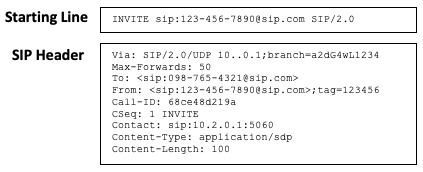
\includegraphics[width=0.7\columnwidth]{chapters/3/img/SIPpacket.png}
    \caption{Example SIP packet}
    \label{f:sippacket}
  \end{center}
\end{figure}


Creating regular expressions for content filtering or pattern matching  is a complex problem that often requires subject matter expertise and manual intervention. Cross-examining multiple packet payloads and examining technical reference documents like RFCs is a time-consuming but necessary process to derive accurate and effective regular expressions. Furthermore, these signatures must be regularly maintained, tested, and updated. Regular expressions become immediately ineffective for example if version numbers are added or changed. In the cybersecurity domain, malware signatures may be easily subverted through simple code or string manipulation so permutations must also be considered. In order to expedite this process and increase signature scope, researchers have leveraged knowledge discovery techniques and applied data mining to extract common features from packet payloads and header contents as input into regular expression signature generation algorithms.

We designed \textsc{Rexactor}, a \textbf{R}egular \textbf{EX}pression \textbf{A}priori \textbf{C}onstruc\textbf{TOR} to extend the state-of-the-art and create more expressive signatures than other solutions are previously capable of generating. \textsc{Rexactor} uses techniques from bioinformatics and natural language processing to encode signatures which use more regex characters and capture more data than previous work while reducing the dynamic memory footprint when employed in regular expression scanning solutions.
